\documentclass[12pt,]{article}
\usepackage{lmodern}
\usepackage{amssymb,amsmath}
\usepackage{ifxetex,ifluatex}
\usepackage{fixltx2e} % provides \textsubscript
\ifnum 0\ifxetex 1\fi\ifluatex 1\fi=0 % if pdftex
  \usepackage[T1]{fontenc}
  \usepackage[utf8]{inputenc}
\else % if luatex or xelatex
  \ifxetex
    \usepackage{mathspec}
  \else
    \usepackage{fontspec}
  \fi
  \defaultfontfeatures{Ligatures=TeX,Scale=MatchLowercase}
\fi
% use upquote if available, for straight quotes in verbatim environments
\IfFileExists{upquote.sty}{\usepackage{upquote}}{}
% use microtype if available
\IfFileExists{microtype.sty}{%
\usepackage{microtype}
\UseMicrotypeSet[protrusion]{basicmath} % disable protrusion for tt fonts
}{}
\usepackage[margin=1.0in]{geometry}
\usepackage{hyperref}
\hypersetup{unicode=true,
            pdftitle={Supplementary Information},
            pdfborder={0 0 0},
            breaklinks=true}
\urlstyle{same}  % don't use monospace font for urls
\usepackage{graphicx,grffile}
\makeatletter
\def\maxwidth{\ifdim\Gin@nat@width>\linewidth\linewidth\else\Gin@nat@width\fi}
\def\maxheight{\ifdim\Gin@nat@height>\textheight\textheight\else\Gin@nat@height\fi}
\makeatother
% Scale images if necessary, so that they will not overflow the page
% margins by default, and it is still possible to overwrite the defaults
% using explicit options in \includegraphics[width, height, ...]{}
\setkeys{Gin}{width=\maxwidth,height=\maxheight,keepaspectratio}
\IfFileExists{parskip.sty}{%
\usepackage{parskip}
}{% else
\setlength{\parindent}{0pt}
\setlength{\parskip}{6pt plus 2pt minus 1pt}
}
\setlength{\emergencystretch}{3em}  % prevent overfull lines
\providecommand{\tightlist}{%
  \setlength{\itemsep}{0pt}\setlength{\parskip}{0pt}}
\setcounter{secnumdepth}{0}
% Redefines (sub)paragraphs to behave more like sections
\ifx\paragraph\undefined\else
\let\oldparagraph\paragraph
\renewcommand{\paragraph}[1]{\oldparagraph{#1}\mbox{}}
\fi
\ifx\subparagraph\undefined\else
\let\oldsubparagraph\subparagraph
\renewcommand{\subparagraph}[1]{\oldsubparagraph{#1}\mbox{}}
\fi

%%% Use protect on footnotes to avoid problems with footnotes in titles
\let\rmarkdownfootnote\footnote%
\def\footnote{\protect\rmarkdownfootnote}

%%% Change title format to be more compact
\usepackage{titling}

% Create subtitle command for use in maketitle
\providecommand{\subtitle}[1]{
  \posttitle{
    \begin{center}\large#1\end{center}
    }
}

\setlength{\droptitle}{-2em}

  \title{\textbf{Supplementary Information}}
    \pretitle{\vspace{\droptitle}\centering\huge}
  \posttitle{\par}
  \subtitle{\textbf{Seasonal Dynamics of Epiphytic Microbial Communities on Marine
Macrophyte Surfaces}}
  \author{}
    \preauthor{}\postauthor{}
    \date{}
    \predate{}\postdate{}
  
\usepackage{times} % Times New Roman font
\usepackage[T1]{fontenc}

\usepackage[none]{hyphenat}

\usepackage{setspace}
\doublespacing
\setlength{\parskip}{1em}

\usepackage{lineno}

\usepackage{pdfpages}

\usepackage{indentfirst}

\usepackage[labelsep=period, labelfont=bf]{caption}
\renewcommand{\thefigure}{S\arabic{figure}}
\renewcommand{\thetable}{S\arabic{table}}
\captionsetup{justification=raggedright,singlelinecheck=false}

\usepackage{pdflscape}
\newcommand{\blandscape}{\begin{landscape}}
\newcommand{\elandscape}{\end{landscape}}

\usepackage{siunitx}
\DeclareSIUnit\molar{\mole\per\cubic\deci\metre}
\DeclareSIUnit\Molar{\textsc{m}}
\DeclareSIUnit\cells{\text{cells}}

\usepackage{caption}
\captionsetup{justification=justified}

\usepackage{float}
\usepackage{booktabs}
\usepackage{longtable}
\usepackage{array}
\usepackage{multirow}
\usepackage{wrapfig}
\usepackage{float}
\usepackage{colortbl}
\usepackage{pdflscape}
\usepackage{tabu}
\usepackage{threeparttable}
\usepackage{threeparttablex}
\usepackage[normalem]{ulem}
\usepackage{makecell}
\usepackage{xcolor}

\begin{document}
\maketitle

\vspace{60mm}

Marino Korlević\textsuperscript{1\(*\)}, Marsej
Markovski\textsuperscript{1}, Zihao Zhao\textsuperscript{2}, Gerhard J.
Herndl\textsuperscript{2,3}, Mirjana Najdek\textsuperscript{1}

\vspace{40mm}

\textsuperscript{\(*\)}To whom correspondence should be addressed:
\href{mailto:marino.korlevic@irb.hr}{\nolinkurl{marino.korlevic@irb.hr}}

1. Center for Marine Research, Ruđer Bošković Institute, Croatia

2. Department of Functional and Evolutionary Ecology, University of
Vienna, Austria

3. Department of Marine Microbiology and Biogeochemistry, Royal
Netherlands Institute for Sea Research, Utrecht University, The
Netherlands

\sisetup{mode=text}
\setlength\parindent{24pt}

\hypertarget{supplementary-figures}{%
\subsection{Supplementary Figures}\label{supplementary-figures}}

\begin{figure}[H]

{\centering 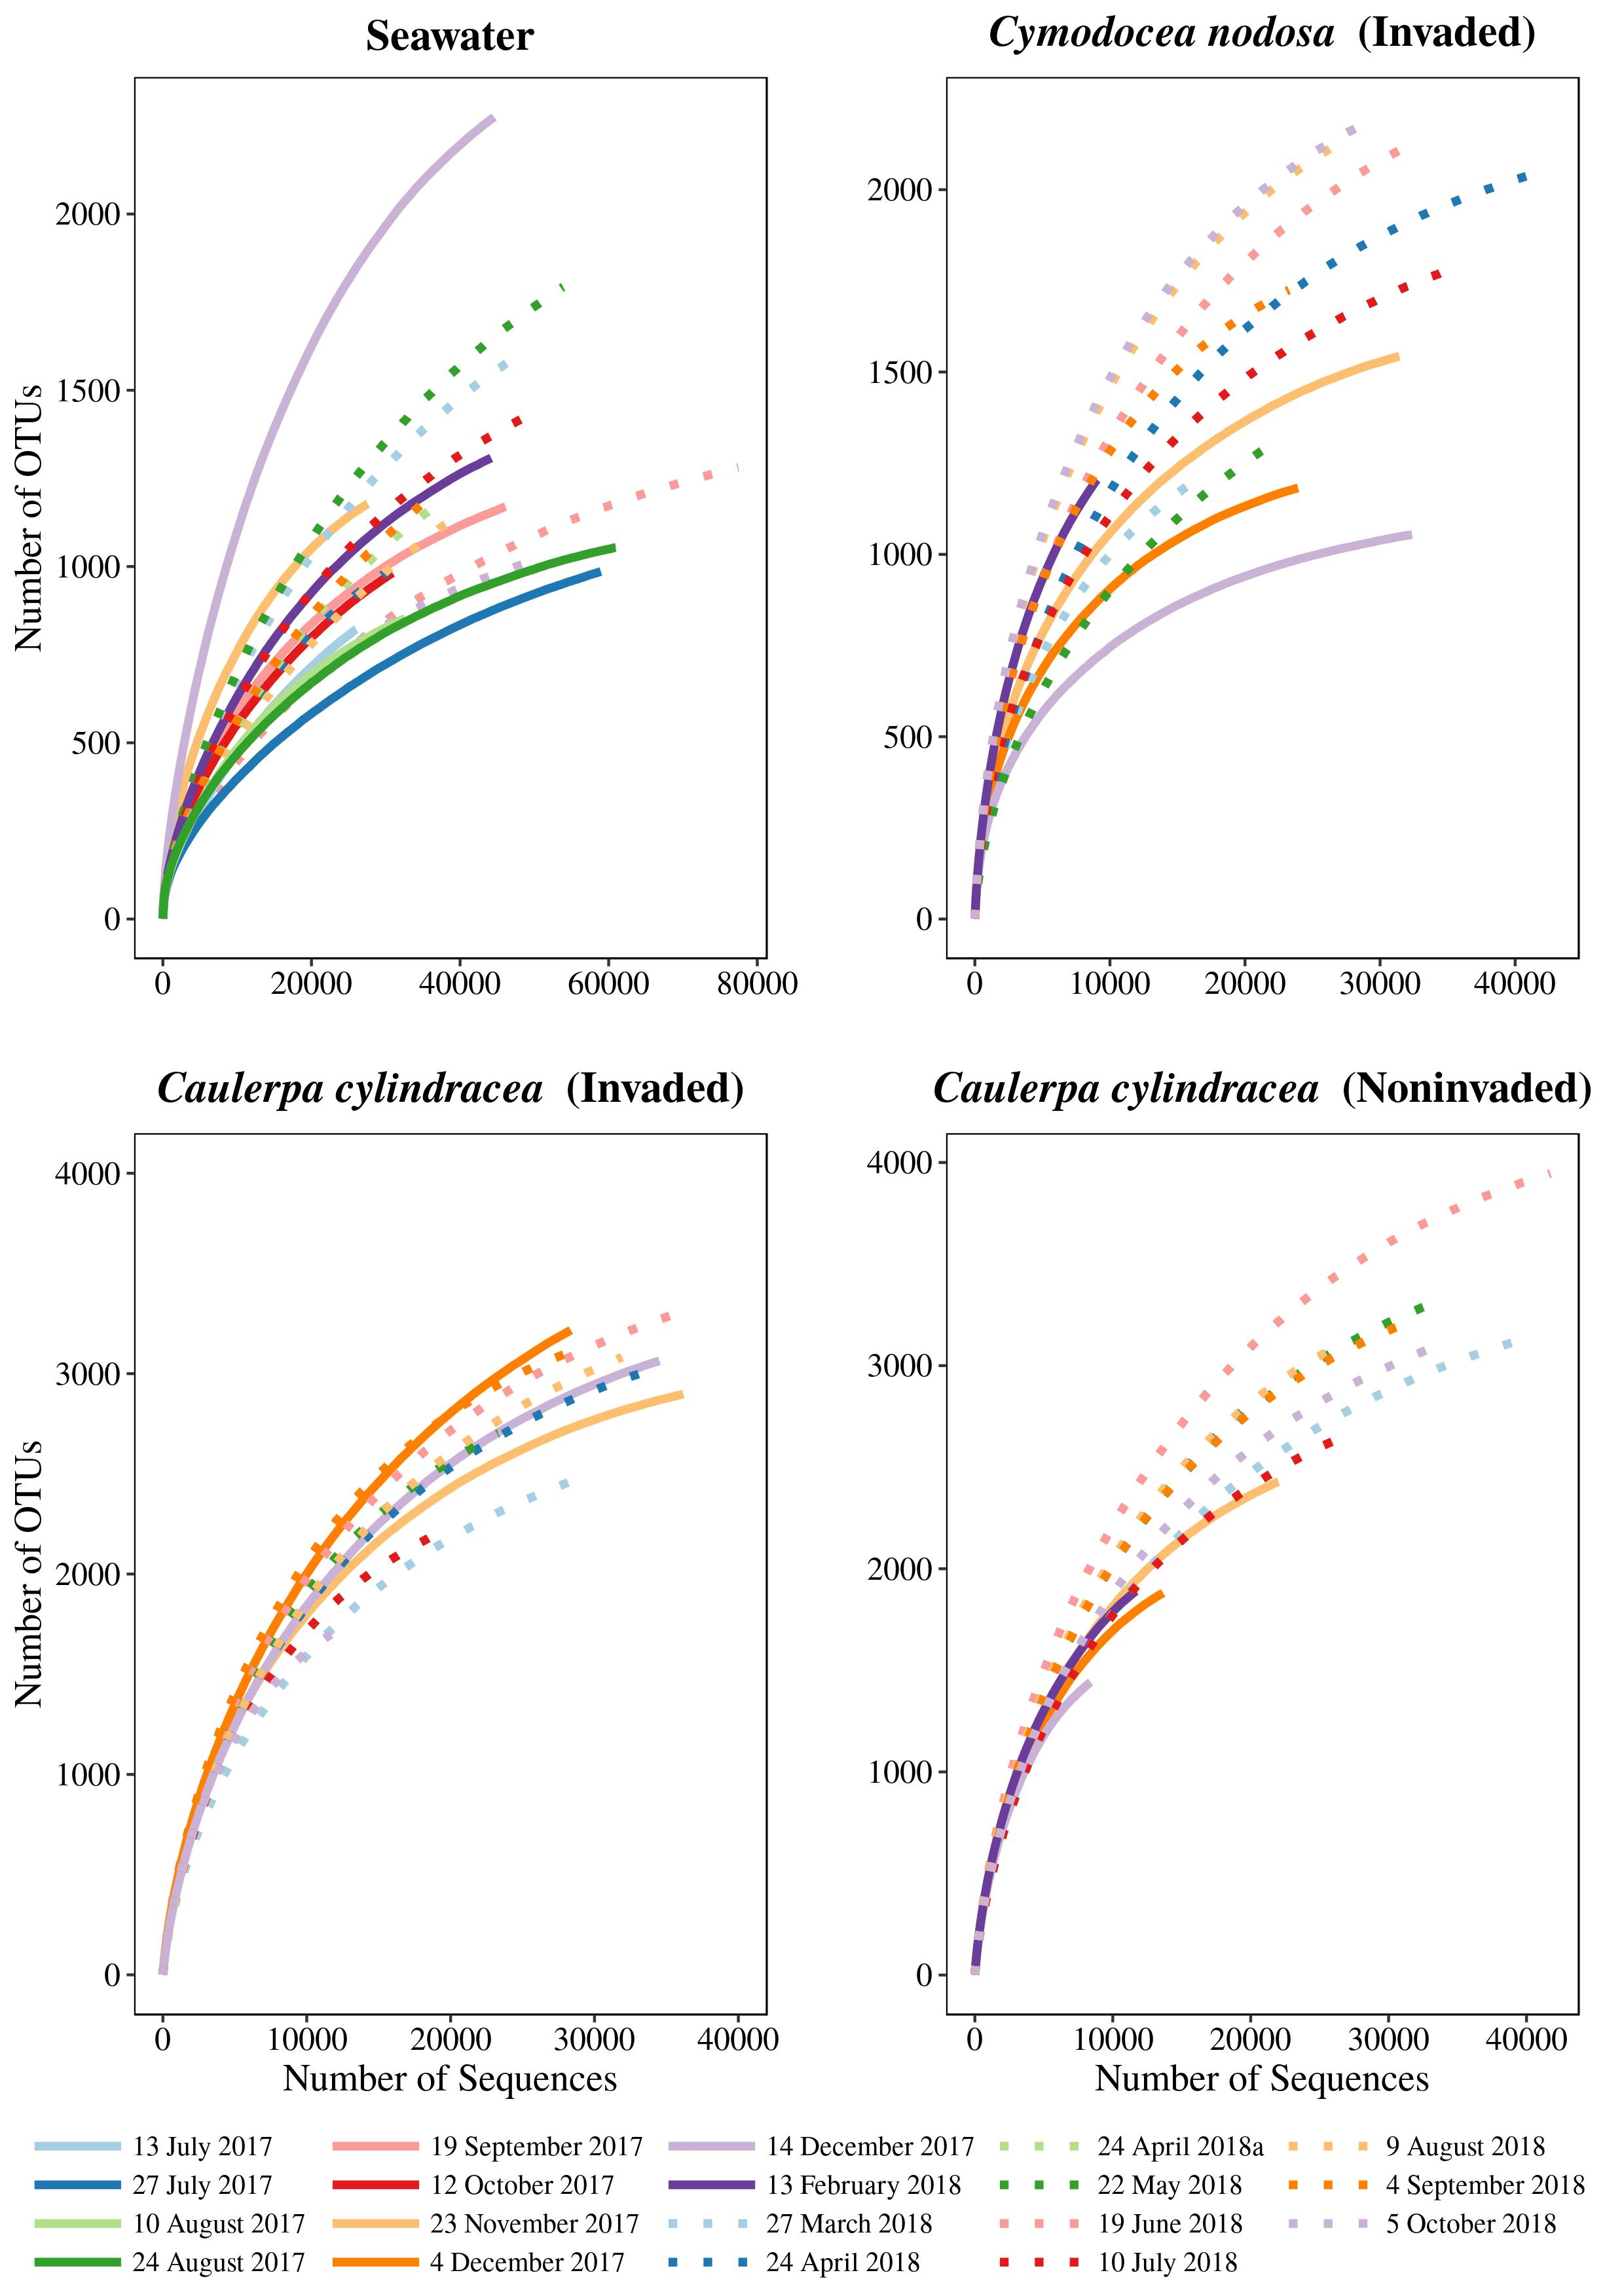
\includegraphics[width=0.85\linewidth]{../results/figures/rarefaction} 

}

\caption{Rarefaction curves of bacterial and archaeal communities from the surfaces of macrophytes (\textit{C. nodosa} [Mixed] and \textit{C. cylindracea} [Mixed and Monospecific]) and in the ambient seawater.\label{rarefaction}}\label{fig:unnamed-chunk-1}
\end{figure}

\begin{figure}[H]

{\centering 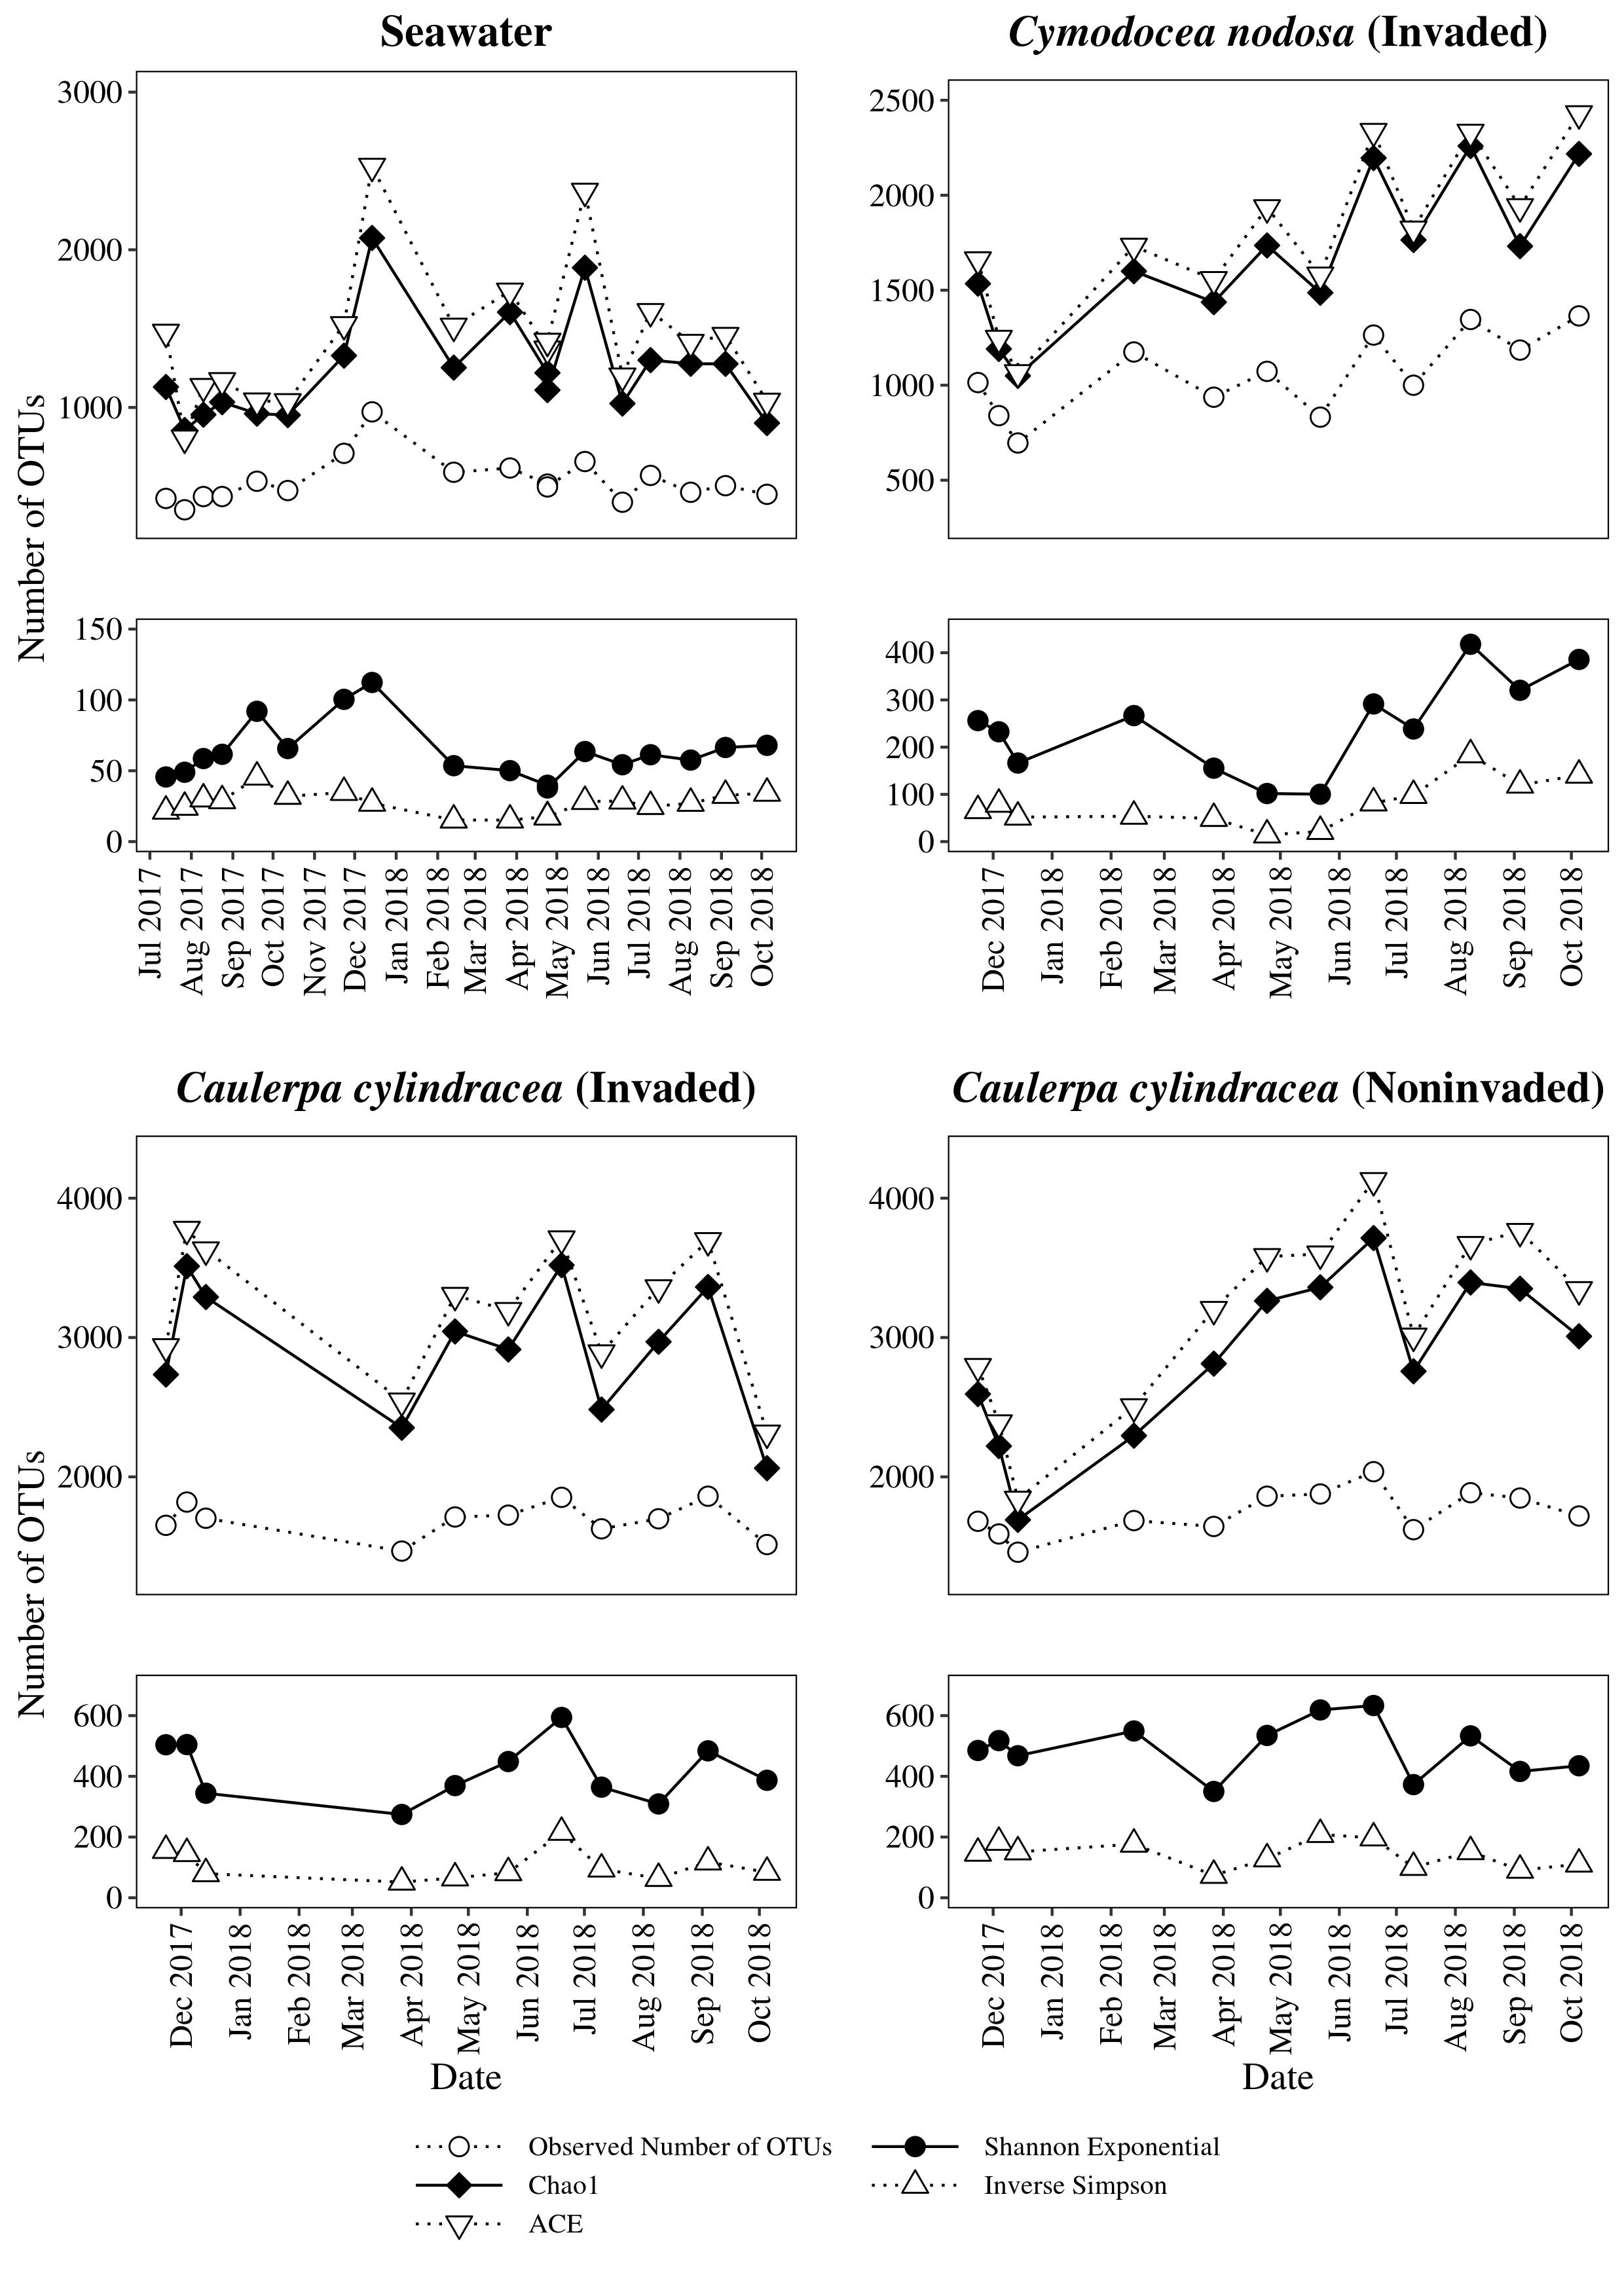
\includegraphics[width=0.85\linewidth]{../results/figures/calculators} 

}

\caption{Seasonal dynamics of observed number of OTUs, Chao1, ACE, exponential of the Shannon Diversity Index and Inverse Simpson Index of bacterial and archaeal communities from the surfaces of macrophytes (\textit{C. nodosa} [Mixed] and \textit{C. cylindracea} [Mixed and Monospecific]) and in the ambient seawater.\label{calculators}}\label{fig:unnamed-chunk-2}
\end{figure}

\begin{figure}[H]

{\centering 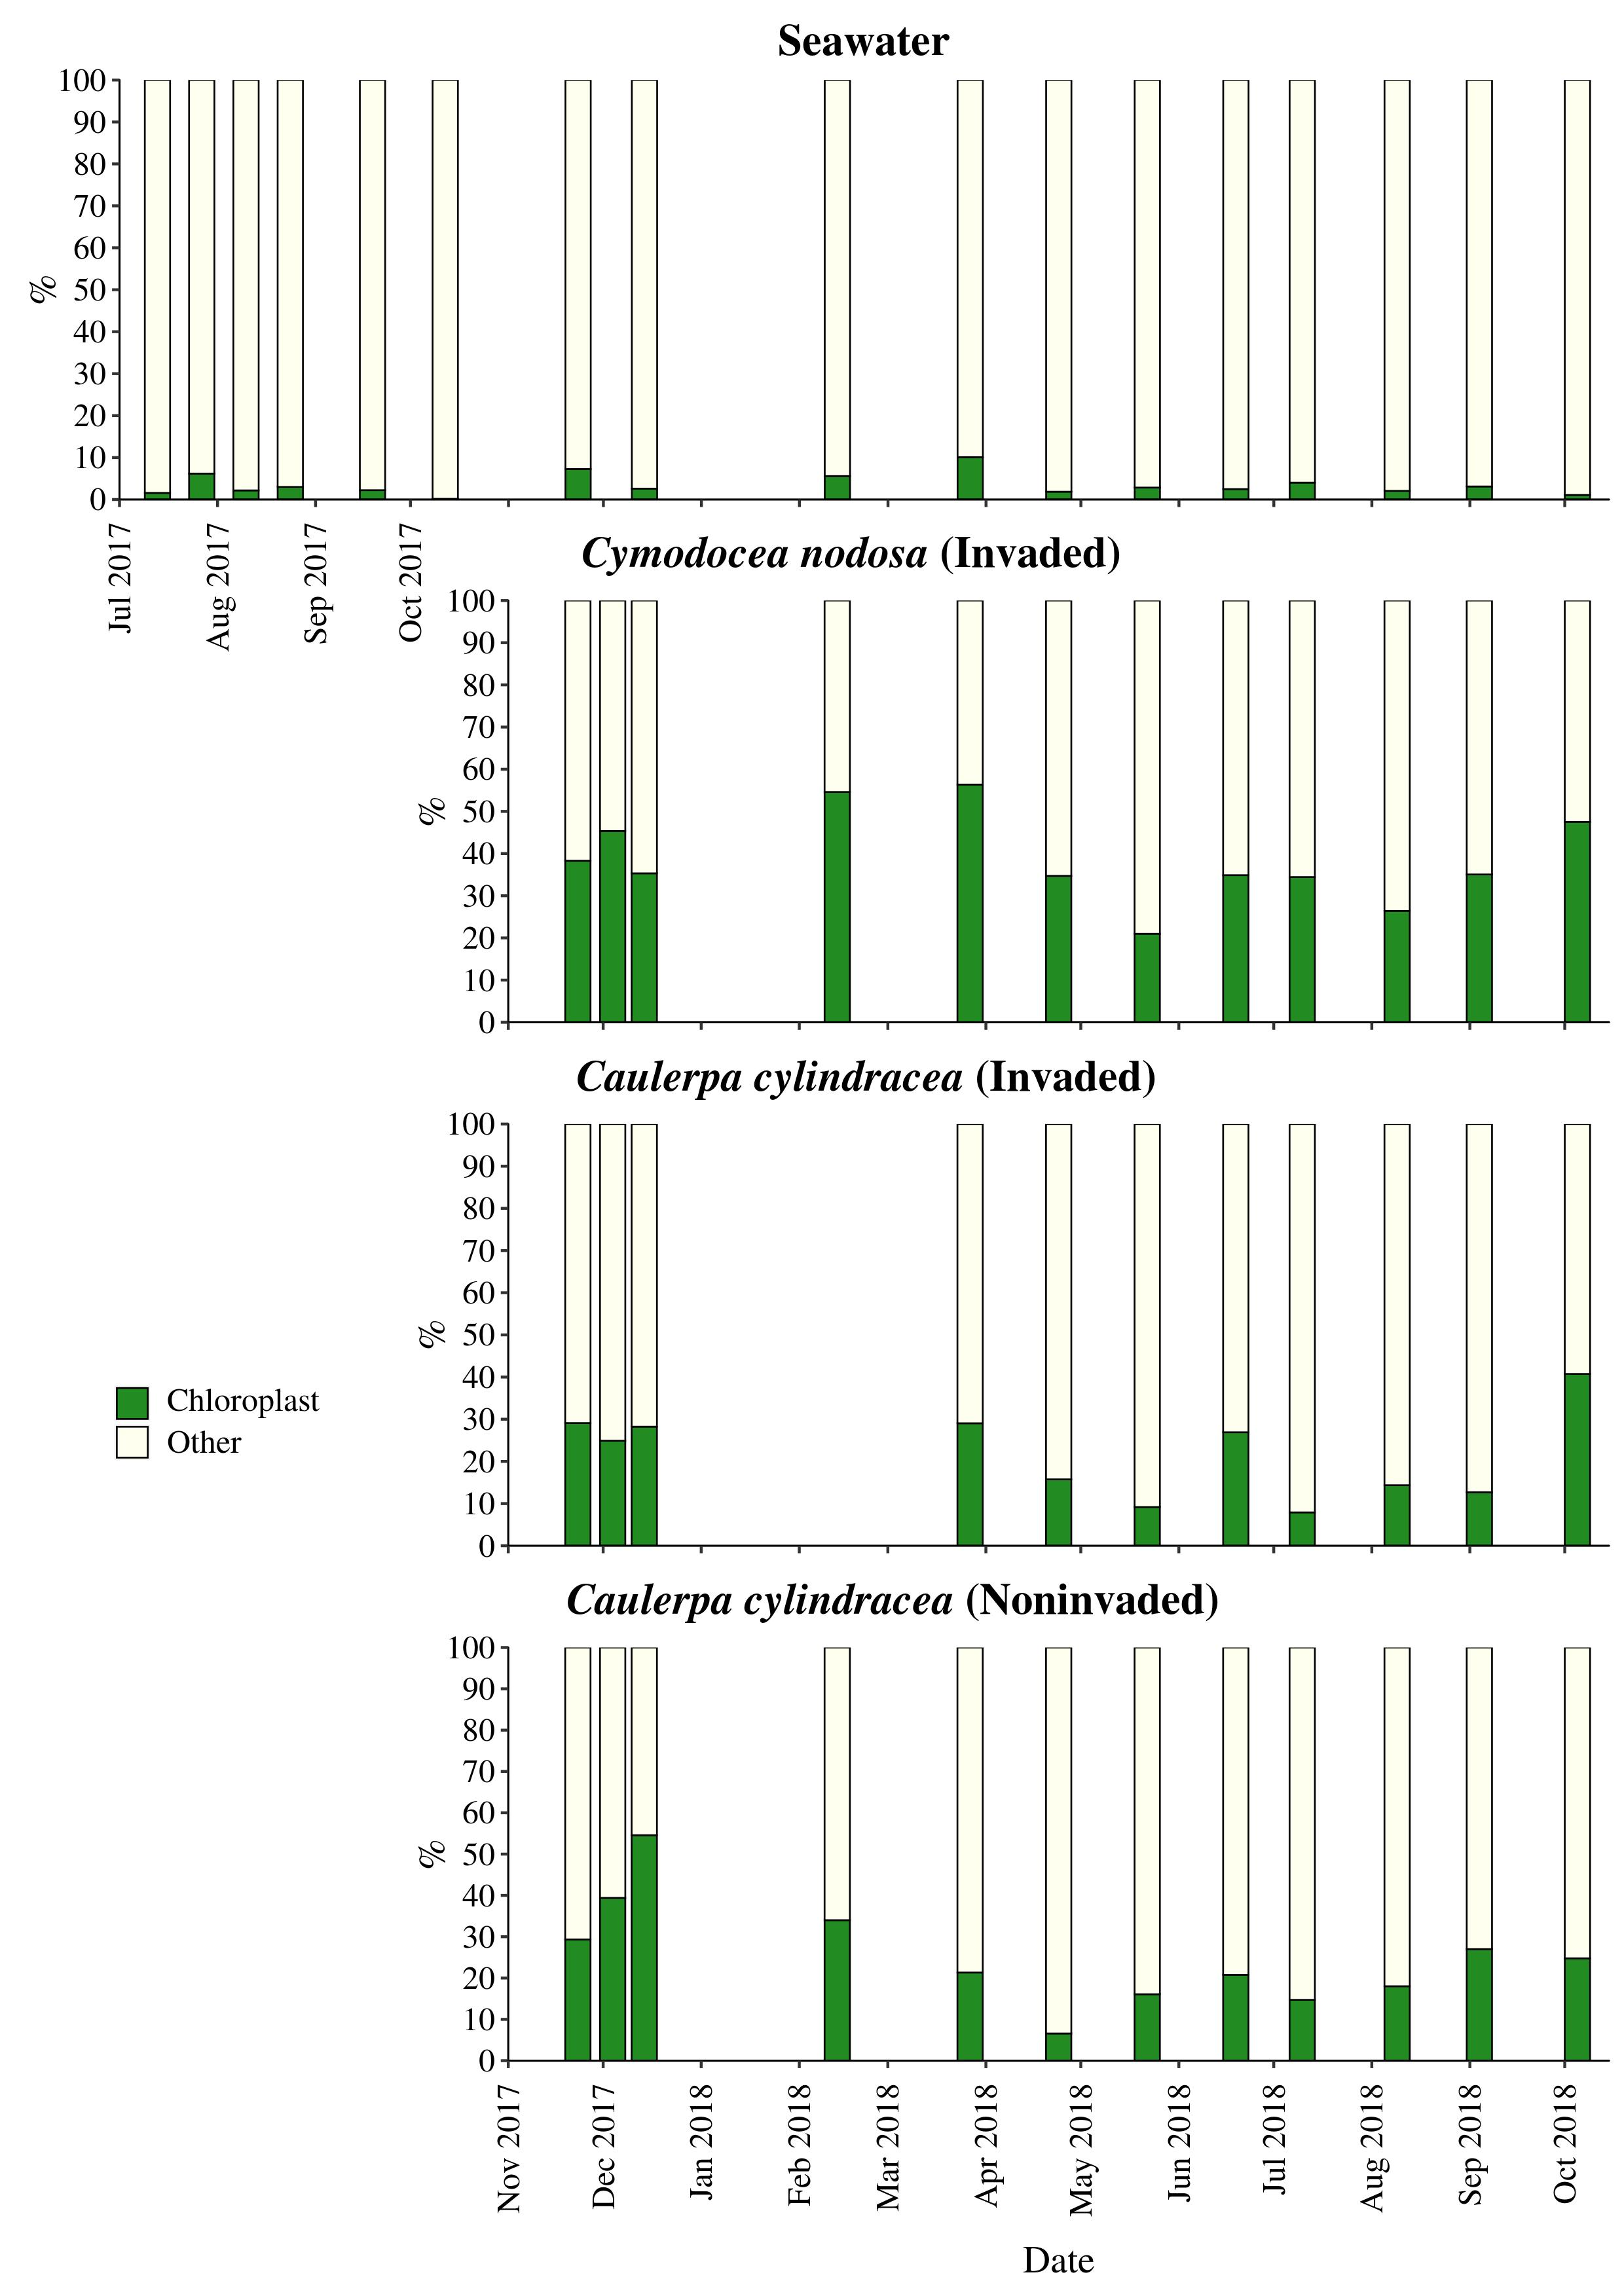
\includegraphics[width=0.85\linewidth]{../results/figures/chloroplast_bar_plot} 

}

\caption{Relative contribution of chloroplast sequences on the surfaces of macrophytes (\textit{C. nodosa} [Mixed] and \textit{C. cylindracea} [Mixed and Monospecific]) and in the ambient seawater.\label{chloroplast}}\label{fig:unnamed-chunk-3}
\end{figure}

\hypertarget{supplementary-table}{%
\subsection{Supplementary Table}\label{supplementary-table}}

\begingroup\fontsize{9}{11}\selectfont

\begin{longtable}[t]{>{\centering\arraybackslash}p{6em}ccccc}
\caption{\label{tab:nseq_notus}Sample ID, Community Type, Sampling Date and Season, No. of Sequences and No. of OTUs of each sample. No. of Sequences and OTUs was calculated after the exclusion of eukaryotic, chloroplast, mitochondrial and no relative sequences.\label{nseq_notus}}\\
\toprule
\textbf{Sample ID} & \textbf{Community Type} & \textbf{Date} & \textbf{Season} & \textbf{No. of Sequences} & \textbf{No. of OTUs}\\
\midrule
\endfirsthead
\caption[]{Sample ID, Community Type, Sampling Date and Season, No. of Sequences and No. of OTUs of each sample. No. of Sequences and OTUs was calculated after the exclusion of eukaryotic, chloroplast, mitochondrial and no relative sequences.\label{nseq_notus} \textit{(continued)}}\\
\toprule
\textbf{Sample ID} & \textbf{Community Type} & \textbf{Date} & \textbf{Season} & \textbf{No. of Sequences} & \textbf{No. of OTUs}\\
\midrule
\endhead
\
\endfoot
\bottomrule
\endlastfoot
3 & Seawater & 13 July 2017 & Summer & 25,996 & 821\\
5 & Seawater & 27 July 2017 & Summer & 58,954 & 993\\
7 & Seawater & 10 August 2017 & Summer & 32,626 & 853\\
9 & Seawater & 24 August 2017 & Summer & 60,935 & 1,064\\
11 & Seawater & 19 September 2017 & Summer & 46,107 & 1,179\\
13 & Seawater & 12 October 2017 & Autumn & 30,911 & 971\\
15 & Seawater & 23 November 2017 & Autumn & 27,585 & 1,197\\
17 & Seawater & 14 December 2017 & Autumn & 44,595 & 2,275\\
19 & Seawater & 13 February 2018 & Winter & 44,207 & 1,306\\
21 & Seawater & 27 March 2018 & Winter & 46,313 & 1,561\\
23a & Seawater & 24 April 2018 & Spring & 30,973 & 999\\
23b & Seawater & 24 April 2018 & Spring & 38,563 & 1,195\\
25 & Seawater & 22 May 2018 & Spring & 53,877 & 1,787\\
27 & Seawater & 19 June 2018 & Spring & 77,465 & 1,290\\
29 & Seawater & 10 July 2018 & Summer & 50,793 & 1,445\\
31 & Seawater & 9 August 2018 & Summer & 39,041 & 1,123\\
33 & Seawater & 4 September 2018 & Summer & 36,206 & 1,206\\
35 & Seawater & 5 October 2018 & Autumn & 49,585 & 1,019\\
37 & \textit{Cymodocea nodosa} (Mixed) & 23 November 2017 & Autumn & 31,237 & 1,555\\
41 & \textit{Cymodocea nodosa} (Mixed) & 4 December 2017 & Autumn & 24,234 & 1,174\\
45 & \textit{Cymodocea nodosa} (Mixed) & 14 December 2017 & Autumn & 32,683 & 1,061\\
49 & \textit{Cymodocea nodosa} (Mixed) & 13 February 2018 & Winter & 9,088 & 1,216\\
52 & \textit{Cymodocea nodosa} (Mixed) & 27 March 2018 & Winter & 17,005 & 1,216\\
55 & \textit{Cymodocea nodosa} (Mixed) & 24 April 2018 & Spring & 42,645 & 2,053\\
58 & \textit{Cymodocea nodosa} (Mixed) & 22 May 2018 & Spring & 21,337 & 1,290\\
61 & \textit{Cymodocea nodosa} (Mixed) & 19 June 2018 & Spring & 31,726 & 2,098\\
64 & \textit{Cymodocea nodosa} (Mixed) & 10 July 2018 & Summer & 35,729 & 1,793\\
67 & \textit{Cymodocea nodosa} (Mixed) & 9 August 2018 & Summer & 26,356 & 2,116\\
70 & \textit{Cymodocea nodosa} (Mixed) & 4 September 2018 & Summer & 23,275 & 1,724\\
73 & \textit{Cymodocea nodosa} (Mixed) & 5 October 2018 & Autumn & 29,907 & 2,211\\
38 & \textit{Caulerpa cylindracea} (Mixed) & 23 November 2017 & Autumn & 36,309 & 2,896\\
42 & \textit{Caulerpa cylindracea} (Mixed) & 4 December 2017 & Autumn & 28,383 & 3,249\\
46 & \textit{Caulerpa cylindracea} (Mixed) & 14 December 2017 & Autumn & 34,718 & 3,067\\
53 & \textit{Caulerpa cylindracea} (Mixed) & 27 March 2018 & Winter & 28,689 & 2,481\\
56 & \textit{Caulerpa cylindracea} (Mixed) & 24 April 2018 & Spring & 34,784 & 3,057\\
59 & \textit{Caulerpa cylindracea} (Mixed) & 22 May 2018 & Spring & 23,392 & 2,712\\
62 & \textit{Caulerpa cylindracea} (Mixed) & 19 June 2018 & Spring & 36,488 & 3,311\\
65 & \textit{Caulerpa cylindracea} (Mixed) & 10 July 2018 & Summer & 18,483 & 2,188\\
68 & \textit{Caulerpa cylindracea} (Mixed) & 9 August 2018 & Summer & 31,943 & 3,097\\
71 & \textit{Caulerpa cylindracea} (Mixed) & 4 September 2018 & Summer & 29,273 & 3,152\\
74 & \textit{Caulerpa cylindracea} (Mixed) & 5 October 2018 & Autumn & 11,707 & 1,711\\
39 & \textit{Caulerpa cylindracea} (Monospecific) & 23 November 2017 & Autumn & 22,057 & 2,428\\
43 & \textit{Caulerpa cylindracea} (Monospecific) & 4 December 2017 & Autumn & 13,661 & 1,892\\
47 & \textit{Caulerpa cylindracea} (Monospecific) & 14 December 2017 & Autumn & 8,409 & 1,451\\
51 & \textit{Caulerpa cylindracea} (Monospecific) & 13 February 2018 & Winter & 11,673 & 1,899\\
54 & \textit{Caulerpa cylindracea} (Monospecific) & 27 March 2018 & Winter & 39,471 & 3,142\\
57 & \textit{Caulerpa cylindracea} (Monospecific) & 24 April 2018 & Spring & 20,304 & 2,836\\
60 & \textit{Caulerpa cylindracea} (Monospecific) & 22 May 2018 & Spring & 33,035 & 3,314\\
63 & \textit{Caulerpa cylindracea} (Monospecific) & 19 June 2018 & Spring & 41,841 & 3,976\\
66 & \textit{Caulerpa cylindracea} (Monospecific) & 10 July 2018 & Summer & 27,038 & 2,669\\
69 & \textit{Caulerpa cylindracea} (Monospecific) & 9 August 2018 & Summer & 26,734 & 3,123\\
72 & \textit{Caulerpa cylindracea} (Monospecific) & 4 September 2018 & Summer & 31,874 & 3,248\\
75 & \textit{Caulerpa cylindracea} (Monospecific) & 5 October 2018 & Autumn & 33,073 & 3,078\\*
\end{longtable}
\endgroup{}


\end{document}
